
\newpage
\sect{Appendix A \quad What does uploading actually fix?}
For a fixed pair of classifiers on identical inputs, a repair is an edge error corrected by the backend. A regression is a correct edge decision spoiled by the backend. Full replacement changes the number correct by repairs minus regressions. The physical board results, CPU edge reference and data-source cohorts have separate denominators.

\begin{center}\small
\begin{tabular}{@{}llrrrr@{}}\toprule
Cohort & Final decision & Correct & Repairs & Regressions & BA (\%)\\\midrule
Board (60) & ESP32-S3 & 53 & -- & -- & 77.08\\
 & MobileNet, 224 px & 55 & 3 & 1 & 82.29\\
 & MobileNet, 112 px & 52 & 3 & 4 & 76.04\\\midrule
Clean PlantDoc (121) & Edge reference & 110 & -- & -- & 80.96\\
 & MobileNet, 224 px & 107 & 3 & 6 & 76.44\\
 & DINO, unweighted & 103 & 2 & 9 & 66.96\\
 & DINO, balanced & 108 & 7 & 9 & 87.31\\\midrule
Cornell (1,821) & Edge reference & 1,464 & -- & -- & 68.34\\
 & MobileNet, 112 px & 1,337 & 67 & 194 & 60.60\\
 & MobileNet, 224 px & 1,455 & 92 & 101 & 67.41\\
 & DINO, unweighted & 1,390 & 110 & 184 & 58.30\\
 & DINO, balanced & 1,556 & 286 & 194 & 83.93\\\bottomrule
\end{tabular}\end{center}
\note{Every Cornell 224-pixel row incurs 12,295,378 JPEG bytes. Sending the 112-pixel versions uses 4,793,088 bytes. The 60 physical records are a subset of the PlantDoc data and are never added to a larger sample count.}

The frozen board and its FP32 counterpart disagreed on one binary decision, where FP32 was correct. Six errors were common to both. Routing the three board abstentions to the FP32 model resolved all three, leaving six errors on the complete batch. Precision escalation alone had little opportunity to repair this cohort. For the 224-pixel MobileNet, the apparent advantage on the small board cohort changes sign on clean PlantDoc and on Cornell.

The strongest intervention at fixed image cost was at the server. On Cornell, balancing the DINO training loss changed the healthy false-positive count from 430 to 101 and the disease false-negative count from 1 to 164. AUROC changed only from 0.927 to 0.930. Much of the practical change is the operating point. With the balanced server and a 10\% uplink budget on Cornell, buffering images and prioritizing edge scores closest to 0.30 yielded 31 additional correct decisions. Cheapest-first lost one. A label-aware selection could gain 186 at this budget. The repository includes 30 random orderings and the full 5--100\% budget sweep.

\subt{How much adjudication establishes the sign?}
After shadow inference, let $D$ be the number of binary disagreements in $N$ records and $R$ the number favouring the remote model. The change in batch accuracy is $(2R-D)/N$. Drawing a fixed uniform sample without replacement from those $D$ records gives an exact hypergeometric interval for $R$. On Cornell, 50 disagreement labels would establish the negative sign for the 112-pixel MobileNet with probability 97.70\%, compared with 13.20\% for 50 uniformly selected frames. For the near-tied 224-pixel MobileNet the same probabilities were only 3.91\% and 0.62\%. These are retrospective design powers conditional on the fully labelled batch. They include no savings in shadow uploads and confer no guarantees on future images.

\newpage
\sect{Appendix B \quad Sending a new decision head}
We group Cornell images by perceptual-hash connected component before sampling. Eighteen additional component members are omitted. A stable hash partitions 1,803 representatives into a 450-image label bank and a 1,353-image holdout containing 377 healthy and 976 diseased images. Each of 20 seeded draws supplies nested samples of 8, 32 and 128 bank images. Every target-assisted method uses exactly those labels. No holdout label is used in fitting or threshold selection. The same holdout is reused across draws, so dispersion measures sensitivity to the choice of calibration images.

A camera can transmit the 1,280-dimensional pre-classifier activation for each labelled image. We quantize activations symmetrically to signed bytes with a per-image scale. The service decodes the records, normalizes the features and fits class-balanced logistic regression. We return a signed-byte weight vector, dimension, scale, bias and format identifier, totalling 1,294 bytes. Training records cost 1,293 bytes each including identifier and label. In comparison, the scalar method fits the original logit margin, the FP32 control transmits full features, and the remote model fits its 384-dimensional DINO head to the same labelled examples. Two eight-label draws contained only one class. A constant prediction was retained in each affected fit.

\begin{center}\small
\begin{tabular}{@{}lrrr|rr@{}}\toprule
&\multicolumn{3}{c}{Mean BA (\%) by label budget} &\multicolumn{2}{c}{128 labels (\%)}\\
Decision rule & 8 & 32 & 128 & Accuracy & AUROC $\times100$\\\midrule
Frozen edge &69.74&69.74&69.74&81.60&76.84\\
Edge margin only &63.59&72.26&72.01&75.27&76.84\\
Adapted edge, INT8 head &68.48&77.35&80.01&82.74&91.64\\
Adapted edge, FP32 head &68.51&77.36&80.03&82.75&91.64\\
Remote DINO, full target head &65.36&77.66&84.51&84.52&92.57\\
Remote DINO, source score recalibrated &76.85&83.25&84.03&83.47&92.54\\\bottomrule
\end{tabular}\end{center}
\note{A source-balanced DINO head needs no Cornell labels and achieves 83.56\% BA on this same holdout. Eight labels were insufficient for the edge update on average. Supplementary files give counts by draw.}

\begin{center}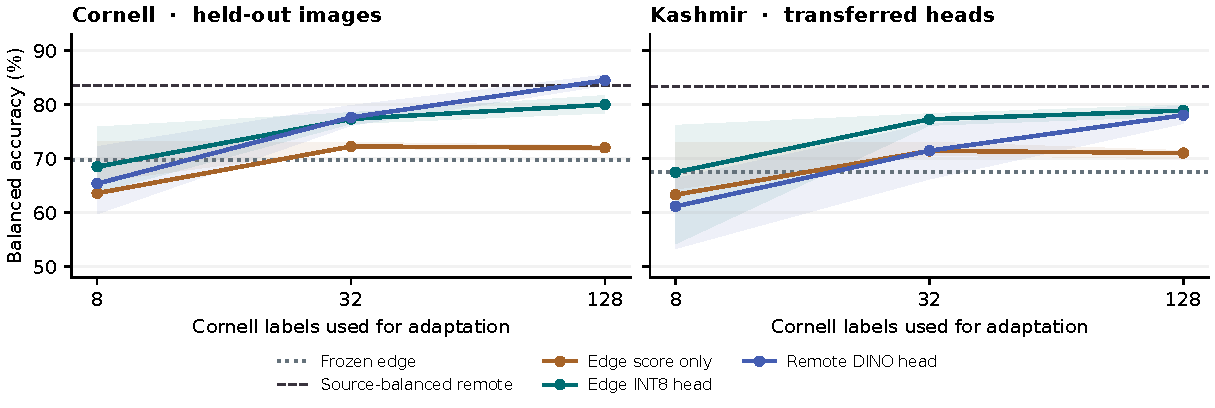
\includegraphics[width=.96\linewidth]{figures/adaptation.pdf}\end{center}
\note{Figure B1. Lines give means over the 20 draws. Shading gives the interquartile range. The same fitted heads are applied unchanged to the processed Kashmir pool. Dashed lines correspond to the source-balanced remote model.}

The INT8 head improves the score ordering. With 128 labels the mean AUROC increases by 14.80 points over the unchanged edge. The one-dimensional edge control retains its prior ordering at 32 and 128 labels. The independent host C99 implementation decoded all 60 packed INT8 heads and matched the Python class decisions on all 81,180 head--image pairs.

\newpage
\sect{Appendix C \quad When does an update use less communication?}
With labels available at the camera, 32 labelled activations and one returned head cost 42,670 bytes. At 128 labels the cost is 166,798 bytes. If a remote reviewer must inspect each calibration photograph, we charge its measured JPEG and identifier as well. The corresponding mean costs are 257,402 and 1,026,890 bytes. The fully remote target-fitted DINO pipeline reuses the same calibration images for review and training and processes every holdout picture. Its mean exchange totals 9,356,348 and 10,001,804 bytes, respectively, including application-level requests and replies. It achieves a higher mean BA at 128 labels. These costs are specific to 1,353 subsequent images.

\subt{A lower bound for the image-based alternative}
To avoid choosing a weak routing baseline, give a router the true class and let it choose the cheapest correcting option on every original edge error. The enlarged menu includes 112- and 224-pixel MobileNet, plus both DINO source heads at 224 pixels. Agreements and regressions can be skipped. Sort correcting payload sizes separately for healthy and diseased edge errors and form prefix costs $C_0(i)$ and $C_1(j)$. With $n_0,n_1$ examples per class, the minimum cost of a BA gain $g$ is
\[
 \min_{i,j}\; C_0(i)+C_1(j) \quad\text{subject to}\quad
               i/(2n_0)+j/(2n_1)\geq g.
\]
For given correction counts the cheapest prefixes attain the minimum, since replacing an expensive correctable image with a cheaper one of its class preserves BA. Enumerating the healthy prefix and the shortest feasible diseased prefix solves the finite problem. Exhaustive assignment on 72 small pools verified the implementation. The comparator even omits network headers and replies, favouring image routing.

\begin{center}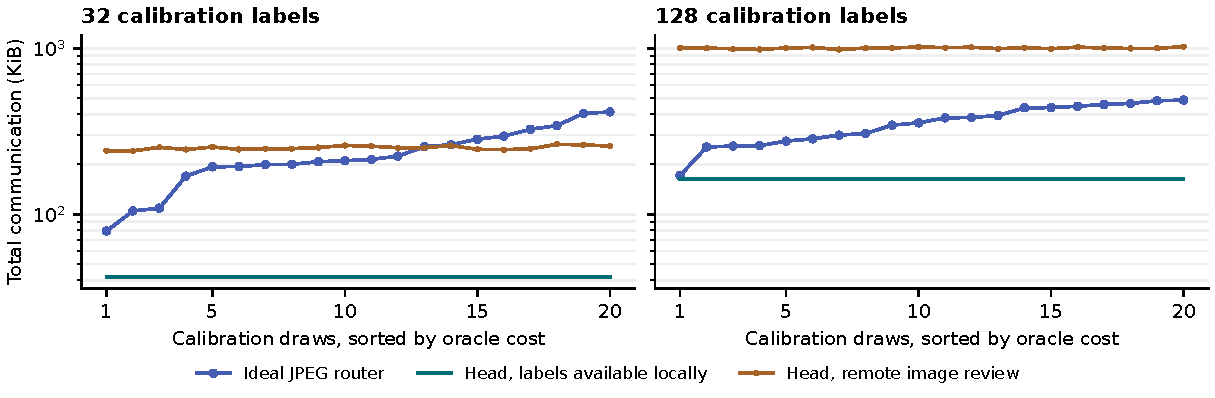
\includegraphics[width=.90\linewidth]{figures/oracle.pdf}\end{center}
\note{Figure C1. Bytes over the entire holdout to match each fitted INT8 head's achieved BA. An oracle can use labels to choose uploads. The two update curves differ only in where calibration images are reviewed.}

At 32 labels the median oracle cost was 217,018 bytes, compared with 42,670 for local review. At 128 it was 376,441 bytes, compared with 166,798. When all labels were available at the camera, the update beat the bound in all 20 draws at both budgets. Sending every calibration image to the annotator changed those counts to 8 of 20 at 32 labels and zero at 128. With 32 of 128 images sent, only 9 of 20 updates remained cheaper, declining to zero with 64 sent. The comparator covers the stated frozen menu and baseline edge. Models with different features, on-camera reweighting, or new encodings would require their own bound.

\subt{Batch service under recorded cellular capacity}
Three paired Mahimahi uplink/downlink traces \cite{mahi} provide 1,500 bytes per opportunity, with five initial phases. For 1,353 pending images, the update finished all 1,200 paired transfers sooner. For one image it won 600, tied 80 and lost 520. On AT\&T driving LTE with remote labels, median service for update versus full review was 8.294 versus 6.879 s (one pending image) or 8.294 versus 87.656 s (1,353). These are capacity-only estimates. Section 6 evaluates RTT, retransmission, outages, processing and deadlines separately.

\newpage
\sect{Appendix D \quad Which operating conditions change the answer?}
\subt{A deployment that prioritizes sensitivity}
The 128-label INT8 head increased healthy specificity from 42.97\% to 73.86\% on Cornell. Disease sensitivity declined from 96.52\% to 86.17\%. An operator for whom a missed lesion is much worse than an extra inspection would value these changes differently. We therefore divide each 128-label draw into 64 fitting and 64 threshold-calibration examples. For each fitted score we choose the largest threshold that accepts at least 95\% of calibration positives, using the inclusive order statistic. Between 41 and 51 positives contributed to each selected threshold.

\begin{center}\small
\begin{tabular}{@{}lrrrr@{}}\toprule
Held-out operation & Sens. (\%) & Spec. (\%) & BA (\%) & Draws at 95\% sens.\\\midrule
Frozen published cutoff &96.52&42.97&69.74&20/20$^{*}$\\
Original margin, calibrated cutoff &94.09&48.62&71.35&9/20\\
INT8 head, default cutoff &86.09&69.95&78.02&0/20$^{\dagger}$\\
INT8 head, calibrated cutoff &94.19&53.28&73.73&11/20\\
DINO target head, calibrated cutoff &92.07&64.97&78.52&2/20\\\bottomrule
\end{tabular}\end{center}
\note{$^{*}$The frozen classifier is repeated unchanged on the common holdout. $^{\dagger}$The default-cutoff entry is taken from the same 64-label fitting experiment as the calibrated entry.}

Adjusting only the original score threshold and fitting a scalar logistic function before thresholding gave identical decisions in all 20 runs. At the calibrated operating point, the adapted edge provided higher mean specificity than the margin-only baseline at similar average sensitivity. Individual fitted-head sensitivities ranged from 86.17\% to 98.57\%. A target sensitivity on the calibration panel did not certify it on the held-out images.

\subt{Transfer without local refitting}
The third collection comprises apple images acquired in Jammu and Kashmir \cite{yatoo}. A pinned public mirror has 5,612 processed rows with three classes. We took the 128 lowest salted filename hashes in each class. The 384 selected files had unique SHA-256 values and no perceptual match within the pool or against 7,191 checked source files, including Cornell. The originating collection uses augmentation, and parent photograph identities are unavailable in the mirror. Counts describe a finite processed-image pool. Sampling equal counts per source class gives twice as many diseased as healthy images in the binary task.

Transferred 128-label INT8 heads achieved 78.91\% mean BA versus 67.58\% for the frozen edge. Specificity rose from 36.72\% to 78.48\%, while sensitivity fell from 98.44\% to 79.34\%. Ordinary accuracy changed from 77.86\% to 79.05\%. A DINO head fitted to the same Cornell labels achieved 78.05\% BA on transfer. The source-balanced DINO model reached 83.40\% with no Cornell labels. These estimates apply to the V2 pipeline with supervision already available. The source-balanced remote model supplies the common expert for the experiments in Sections 3--5.

\subt{Scope of the device and network measurements}
Archived hardware validates the starting device model for only one fixed cohort. The preceding experiment fitted and evaluated heads on features of the frozen FP32 graph. Section 6 quantifies sensitivity to its numerical approximation. Their compute and energy on the deployed INT8 backbone remain unmeasured. Image-source labels are proxies for visible abnormality, with unknown plant-level groupings. Measured payloads and historical network traces support communication comparisons. Neither establishes end-to-end field latency, disease prevalence, yield improvement or effects of acting on an alert. For this camera and these collections, the operational choice turns on the reviewer location, cost of a miss, and number of future images over which one can amortize an update.

\newpage
\sect{Appendix E \quad Retrospective batch scheduling with local supervision}
An updated edge classifier can change both its answers and the order in which it asks for help. We gave every strategy the same ceiling in application bytes. A review transmits a real 224-pixel JPEG and 20 bytes of request and reply fields to the same frozen PlantDoc-balanced DINO service. Unqueried images keep their edge decisions. The original camera queues frames closest to its released 0.30 cutoff. The updated camera queues frames with the smallest absolute distance from its new logit cutoff of zero. The sender knows JPEG lengths after encoding and can buffer the batch. A frame is skipped if it does not fit in the remaining allowance. The scheduler sees no evaluation label or remote prediction before making that choice.

For this historical batch comparison we fixed a ceiling of 25\% of the bytes for full review, with 10\% and 50\% for sensitivity. The 20 Cornell-trained 128-label heads in Appendix~B are reused without refitting. We charge the complete calibration and deployment cost to each cohort, including both transfers. If an update cannot fit, the combined system uses the original edge router. The table assumes the 128 reference labels are available at the camera during Cornell calibration.

\begin{center}\small
\begin{tabular}{@{}lrrr@{}}\toprule
Mean BA (\%), 25\% ceiling unless marked & Cornell & Kashmir & Latvia\\\midrule
Frozen server on every image (100\% ceiling) &83.56&83.40&60.64\\
Original edge &69.74&67.58&46.90\\
Original edge + selective review &72.62&76.37&51.54\\
Updated edge alone &80.01&78.91&52.11\\
Updated edge + random review &80.85&79.75&54.55\\
Updated edge + selective review &\textbf{87.06}&\textbf{84.28}&\textbf{54.74}\\\bottomrule
\end{tabular}\end{center}
\note{Latvia uses the presence of visible scab as its endpoint. The random control uses 20 fixed image orderings for each of the 20 head draws and pays the same setup cost. Selective review used means of 283, 75 and 272 uploads (rounded).}

\begin{center}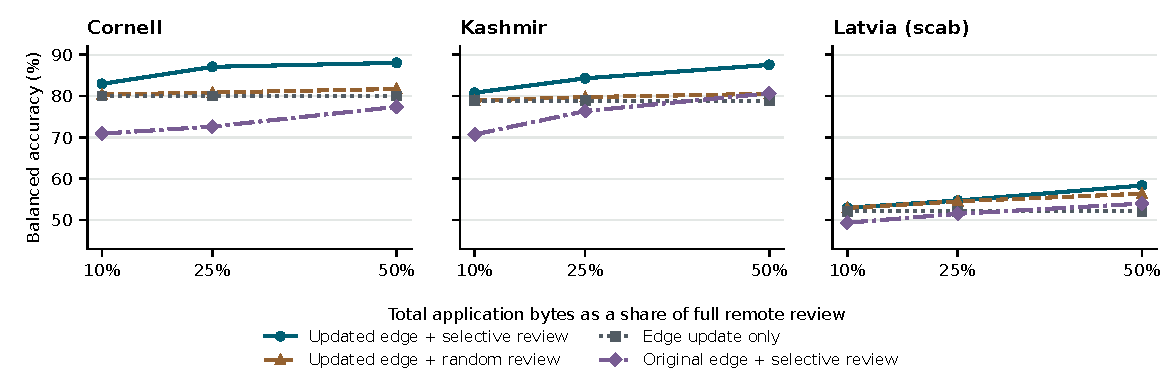
\includegraphics[width=.96\linewidth]{figures/collaboration.pdf}\end{center}
\note{Figure E1. Each cohort uses its own byte ceiling. Each mean reuses a single evaluation pool across draws. The line for the update alone falls back to the original camera if the update cannot fit.}

On Cornell and Kashmir, every calibration draw beat both single interventions at 25\%. The selective policy corrected 100.45 and spoiled 33.35 Cornell decisions per draw, compared with the updated edge alone. On Kashmir these values were 24.65 and 8.20. On Latvia the selective and random policies were within 0.19 points, and only 10 of 20 draws beat mean random review. The service corrected 51.45 decisions and spoiled 91.55 on average there. With 207 negatives and 983 positives there, ordinary accuracy fell from 73.70\% for the original camera to 48.67\% for the joint policy. Mean scab misses rose from 118 to 536.35.

If the Cornell calibration photographs must be transmitted for annotation, joint BA at 25\% becomes 84.76\%, 76.37\% and 53.70\%, respectively. On Kashmir the mean calibration exchange alone exceeded the entire 945,647-byte allowance in every draw. Paying for the labels eliminates the update at this ceiling.

\newpage
\sect{Appendix F \quad Can full review reduce false alarms and misses together?}
Changing one cutoff on a fixed ordering adds or removes alerts in a single direction. To examine two independent changes, we allowed the source-balanced remote model to rescue an edge-negative image and to retract an edge-positive alert. A 475-rule grid was fixed before examining results for this policy. We used the 450 Cornell calibration images to require at least a halving of the 15 original misses and fewer than the 83 original false positives. Four rules qualified. Prespecified tie-breaking first minimized false positives. The selected rule yielded 60 false positives and five misses on calibration. Earlier methods had already been evaluated on the Cornell and Kashmir test collections.

The selected rule queried every photograph. For an original negative it issues an alert if the service's estimated disease probability is at least 0.50. For an original positive it clears the alert only below 0.30. Fitting required 3,031,861 calibration bytes, followed by a 22-byte configuration. All deployments below replay the very same configuration.

\begin{center}\small
\begin{tabular}{@{}lrrr@{}}\toprule
Source and reference counts & False positives & False negatives & Inference bytes\\\midrule
Cornell (377 negative, 976 positive) &$215\to137$&$34\to19$&9,141,584\\
Kashmir (128 negative, 256 positive) &$81\to25$&$4\to25$&3,782,589\\
Latvia (207 negative, 983 positive) &$195\to83$&$118\to334$&10,788,080\\\bottomrule
\end{tabular}\end{center}

The Cornell rule corrected 108 false alarms and 25 missed cases, while introducing 30 false alarms and 10 misses. Much of its net rescue came from scab, where misses fell from 21 to four. Among 67 images with multiple diseases, misses increased from one to four. In Kashmir, 22 of the 24 introduced misses occurred on Alternaria. Only three originally missed Kashmir cases were rescued. These counts come from the same image decisions and distinguish the type of mistake that moved the average.

\subt{Competing choices of representation and operating point}
On Cornell, a single 448-pixel JPEG with three DINO views, fitted on 300 Cornell examples and thresholded on the remaining 150 calibration examples, yielded 83 false positives and 38 misses at a cost of 26,528,371 inference JPEG bytes. On Kashmir it yielded four and 75 respectively. On Latvia it yielded 37 and 401. A preselected two-score fusion yielded 120/39, 22/33 and 64/404, respectively (false positives/misses). Using more pixels or adding two scores can suppress false alarms while losing the intended sensitivity.

Two of 20 earlier high-sensitivity INT8 heads (draws 2 and 4) reduced both counts on both Cornell and Kashmir. They were identified after examining those results. Both were then fixed for Latvia, where their error counts were 192/126 and 181/164, respectively, against the original 195/118. Conditional selection would have overstated their portability.

A stronger single-expert control received the identical 450 labels and considered every distinct observed remote-score cutoff and its endpoints. Under the common calibration constraint of at most seven misses it selected 0.33966 (63 false positives and five misses). In full review it gave 173/18 on Cornell, 25/34 on Kashmir and 62/359 on Latvia. Against this control, the directional combination eliminated nine further misses at unchanged false positives on Kashmir. In Latvia it exchanged 21 additional false positives for 25 fewer misses. The fixed 0.50 remote model also retained higher Cornell BA than the directional combination (83.56\% versus 80.86\%). Threshold comparisons and both single-score controls are included in the artifact. The two-score rule's value depends on the cost assigned to each error.


\newpage
\sect{Appendix G \quad External scab screening and local recalibration}
AppleScabLDs contains all 1,190 leaf photographs in the specified Latvian archive \cite{kodors}, with 207 publisher-negative and 983 visible-scab references. An image without visible scab can show other damage. Photographs include repeated leaf views. An independent ZIP traversal verified all paths, SHA-256 values, labels and perceptual hashes. No exact or perceptual match within Hamming distance five was found against 7,575 archived source images. In the Latvian archive, one member per same-label component at distance four yields 1,148 representatives. The fixed Cornell rule changes false positives from 191 to 81 and misses from 116 to 324 on this subset. Neither perceptual grouping nor spatially distinct collections establishes leaf-level statistical independence.

All images retained original capture dates over 14 days. We reserved the earliest five full days for calibration and all nine later days for evaluation, before looking at the new predictions. No exact or screened near-duplicate component crossed these two partitions. The five days supplied 611 images and labels, including 476 with scab. The later days contained 72 negatives and 507 positives. The date split therefore required substantially more calibration images than a one-third split of individual files.

The identical 475-rule procedure found no candidate that halved calibration misses while lowering false positives. Its prespecified fallback chose among the 38 rules that strictly lowered both. It changed early error counts from 128/69 to 126/56. On the 579 later images the baseline had 67 false positives and 49 misses. The Cornell rule yielded 30 and 159. The rule calibrated on the five local dates yielded 67 and 33. It rescued 18 missed scab images and incorrectly withdrew two true alerts. Sensitivity rose from 90.34\% to 93.49\%, while specificity remained 6.94\%. The early labels and rule installation cost 5,497,944 bytes, followed by 1,554,379 bytes for 175 later queries. This is a within-season analysis with a small later negative cohort.

\begin{center}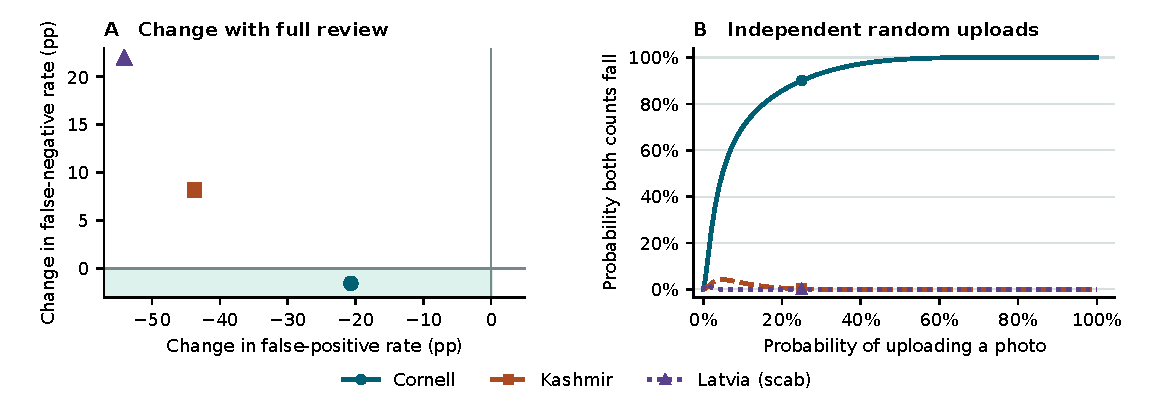
\includegraphics[width=.96\linewidth]{figures/joint_errors.pdf}\end{center}
\note{Figure G1. Left, the shaded quadrant denotes strictly fewer errors in both classes. Right, for a fixed set of scored images, the only randomness is an independent decision to upload each eligible image with probability $q$. At $q=1$ all eligible images get the full-review treatment.}

If full review fixes $a$ and spoils $b$ decisions of one true class, independently sampling eligible uploads with probability $q$ gives a strict improvement probability $P[\mathrm{Bin}(a,q)>\mathrm{Bin}(b,q)]$ for that class, using two independent binomials. The two class-specific events involve disjoint uploads, so their probabilities multiply. At $q=0.25$ the probability of a strict joint reduction is 90.05\% on the fixed Cornell batch and 0.23\% on the fixed Kashmir batch. This retrospective calculation quantifies routing randomness. It assumes no probability law for new leaves.
